\documentclass{beamer}

\usepackage{graphicx}
\usepackage{mathtools}
\usepackage{mathrsfs}

%Information to be included in the title page:
\title{Statistical and Causal Models}
\author{Congyuan Duan}
%\institute{School of Mathematics, Sun Yat-sen University}



\begin{document}

\frame{\titlepage}

\begin{frame}
    \frametitle{Contents}
    \tableofcontents
\end{frame}

\section{Probability Theory and Statistics}

\begin{frame}
    \frametitle{Contents}
    \tableofcontents[currentsection]
\end{frame}

\begin{frame}
    \frametitle{Probability Theory and Statistics}
    \begin{itemize}
        \item[$\bullet$]Probability Theory: Reason about the outcomes of random
        experiments, given the preceding mathematical structure.
        \item[$\bullet$]Statistical Learning: Given the outcomes of experiments, 
        infer properties of the underlying mathematical structure.
    \end{itemize}
\end{frame}

\section{Learning Theory}

\begin{frame}
    \frametitle{Contents}
    \tableofcontents[currentsection]
\end{frame}

\begin{frame}
    \frametitle{Difference}
    \begin{itemize}
        \item[$\bullet$]Infer structure rather than distribution
        \item[$\bullet$]Different training and testing distributions
    \end{itemize}
\end{frame}

\section{Causal Modeling and Learning}

\begin{frame}
    \frametitle{Contents}
    \tableofcontents[currentsection]
\end{frame}

\begin{frame}
    \frametitle{Relationship}
    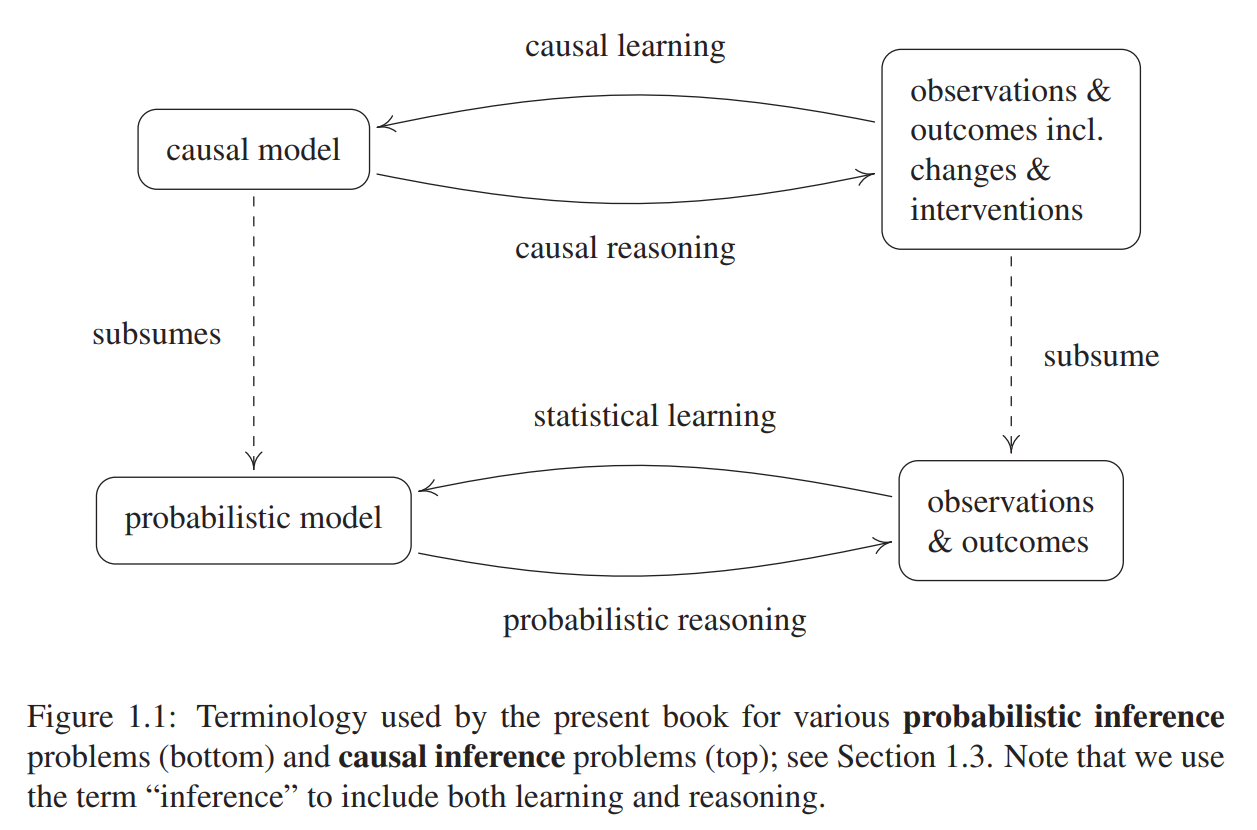
\includegraphics[scale=0.6]{fig3.png}
\end{frame}

\begin{frame}
    \frametitle{Reichenbach's common cause principle}
    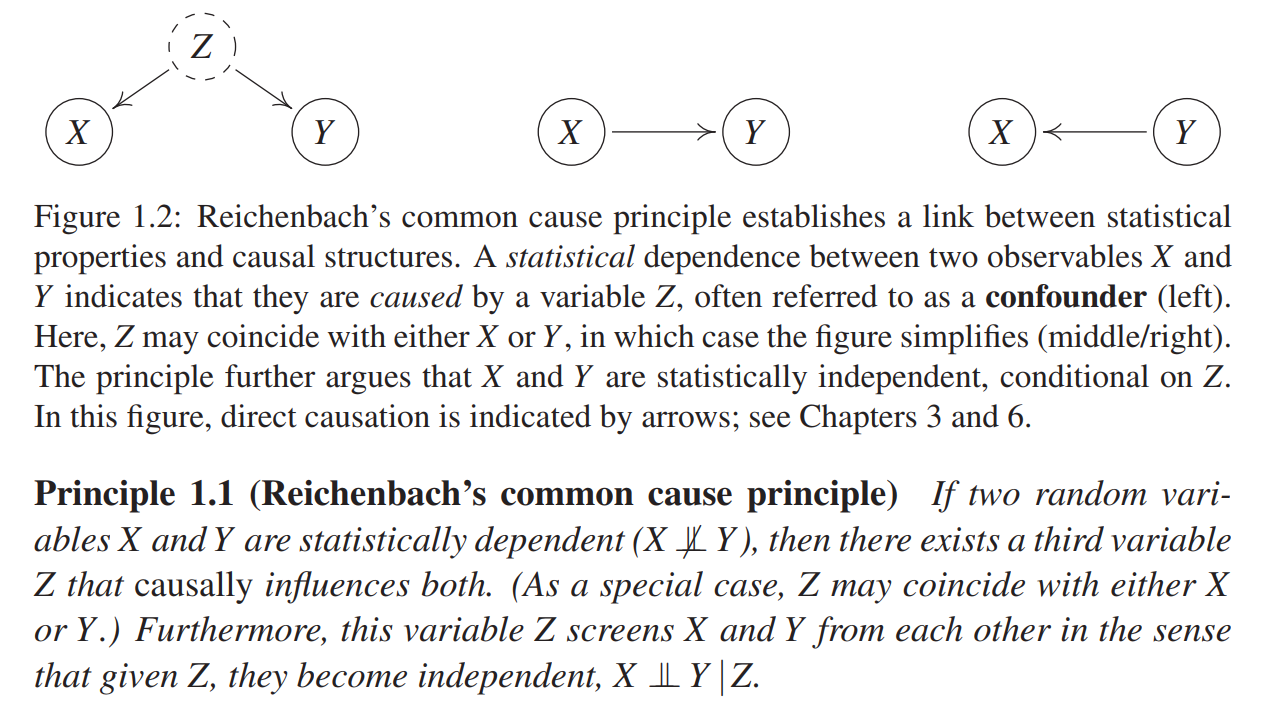
\includegraphics[scale=0.6]{fig1.png}
    Correlation does not imply causation.
\end{frame}

\section{Example}

\begin{frame}
    \frametitle{Contents}
    \tableofcontents[currentsection]
\end{frame}

\begin{frame}
    \frametitle{Optical Character Recognition}
    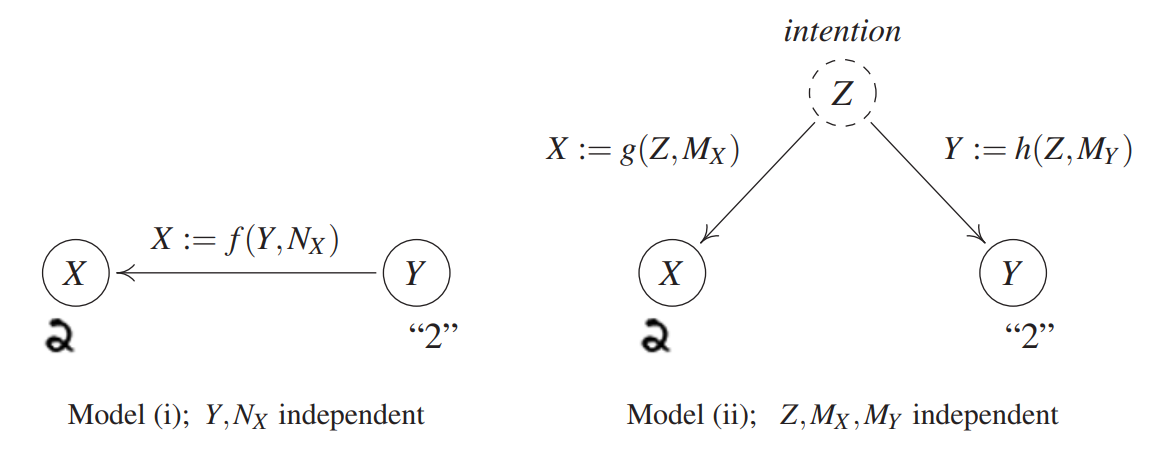
\includegraphics[scale=0.6]{fig2.png}
\end{frame}


\end{document}
